\yesmargins

\chapter{Monolith vs. Microservices Architectures}
\chaptermark{Monolith vs. Microservices}

\begin{tikzpicture}[overlay,remember picture] 
\node[anchor=south] at ([yshift=5in,xshift=0.85in]current page text area.south){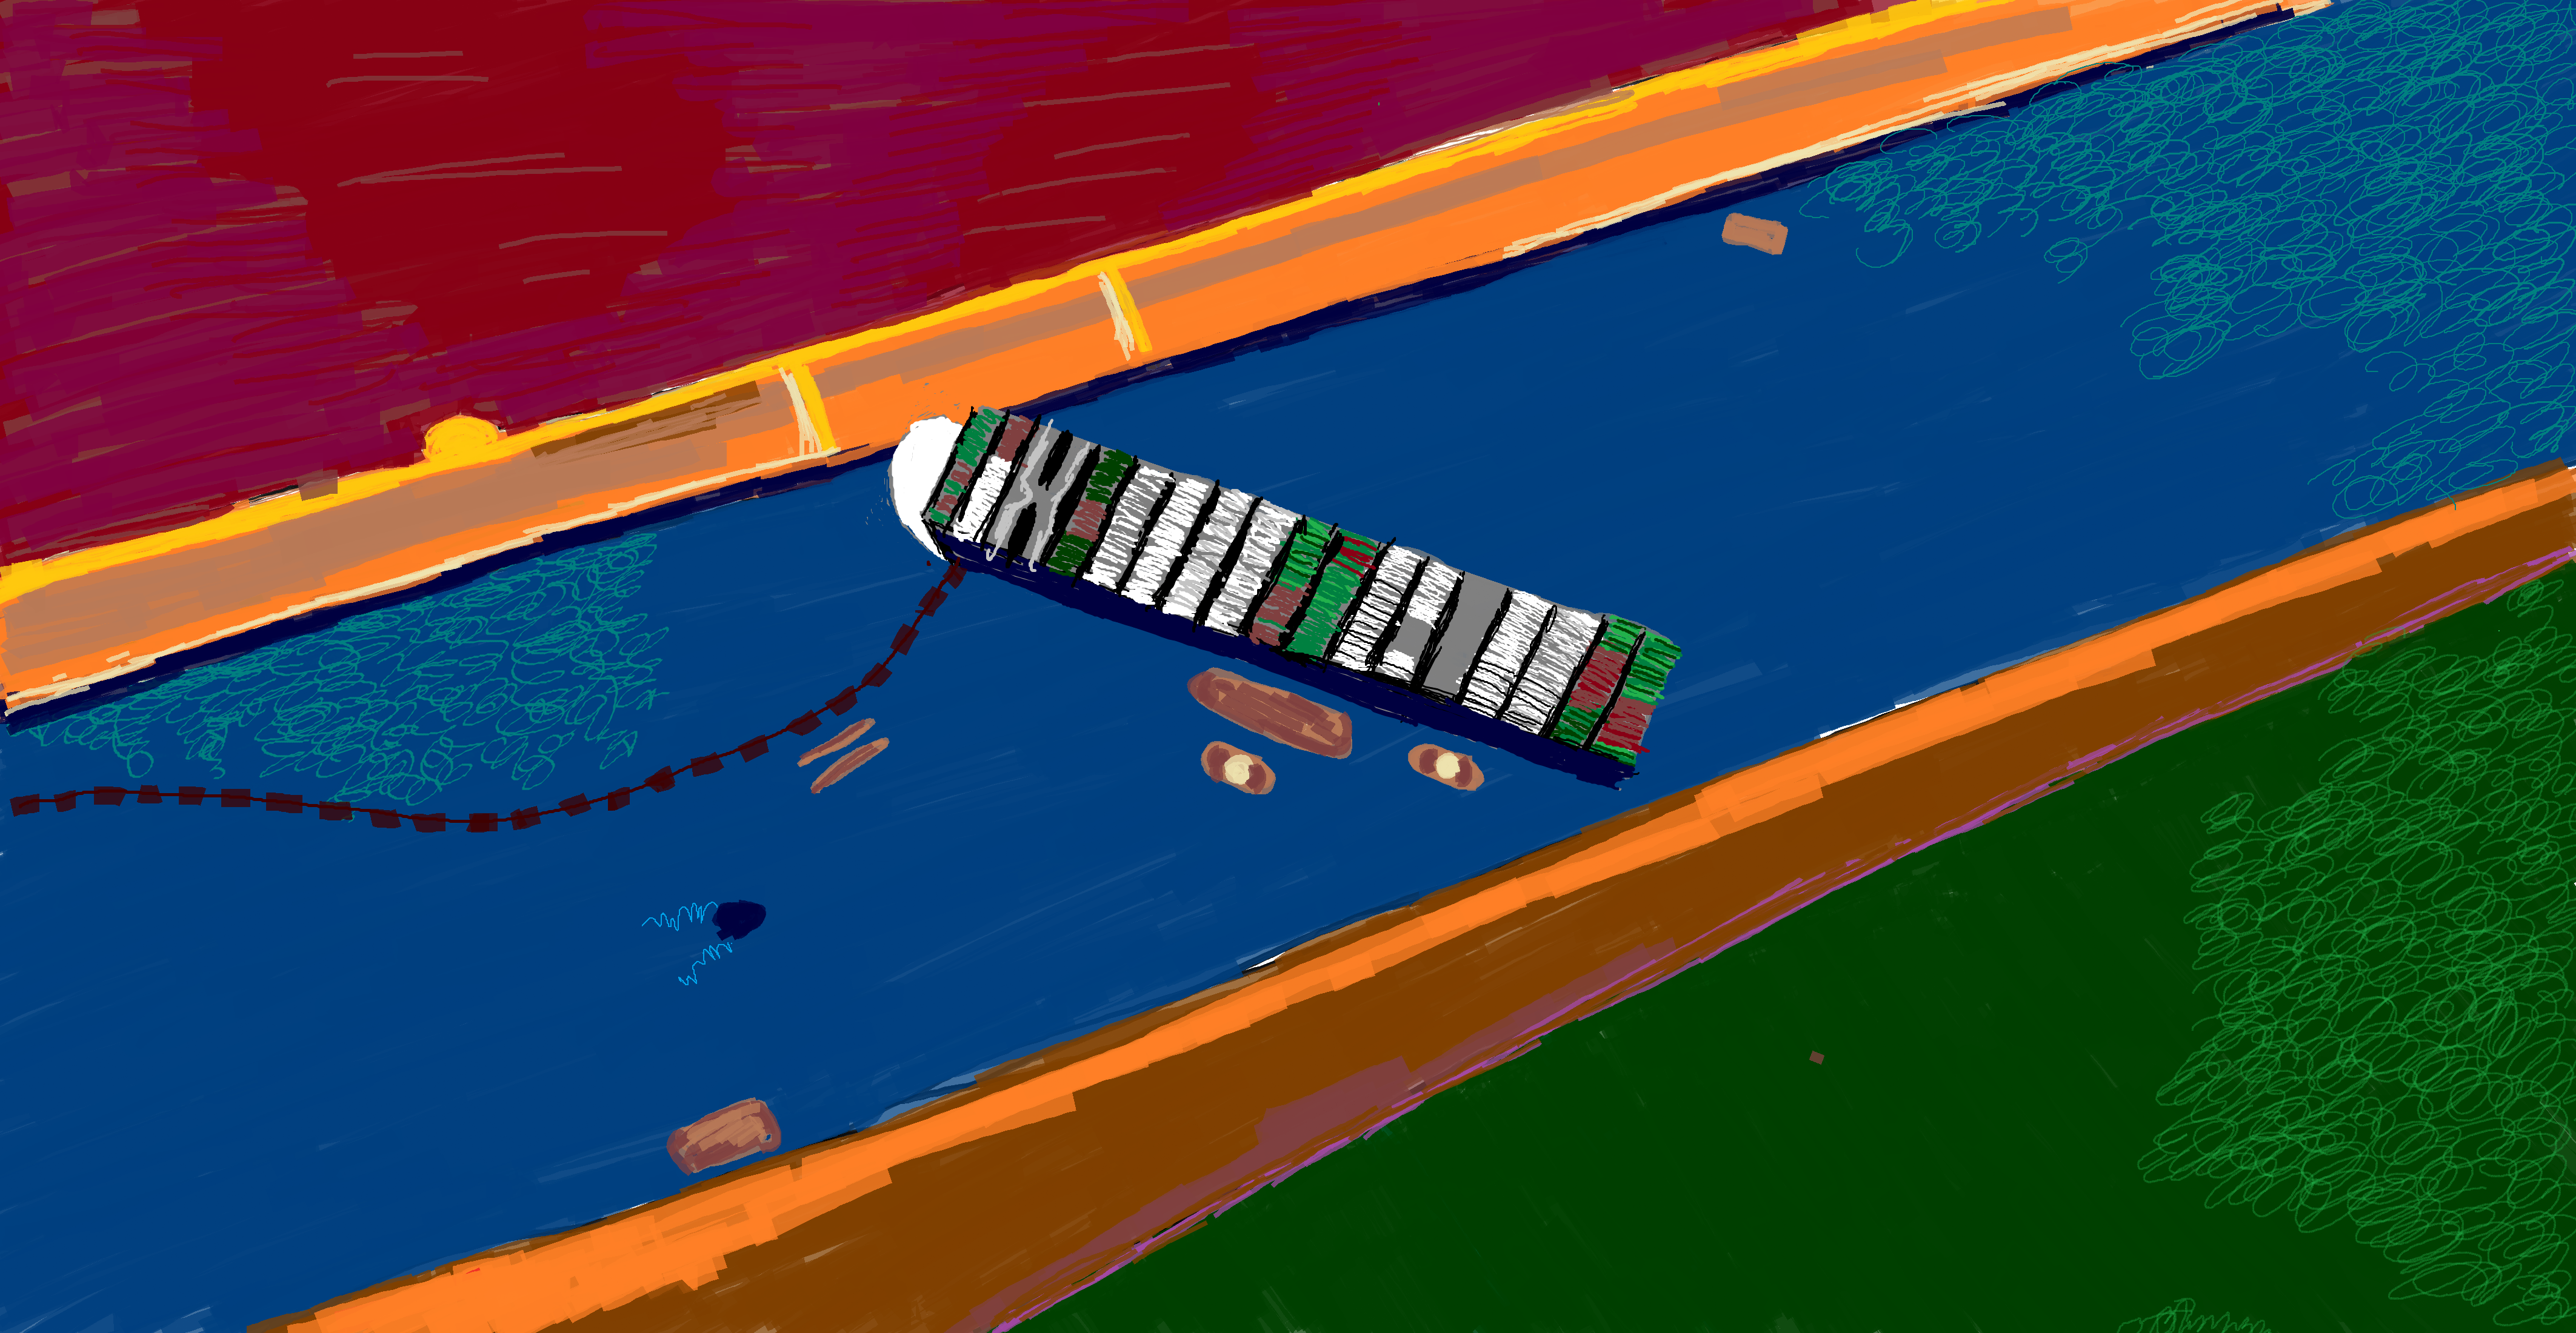
\includegraphics[width=9.5in]{msa05}}; 
\end{tikzpicture}

\marginpar{\softwareArchitectureDef\margindivider}

\marginpar{\highLevelArchitectureDef}

\textbf{High-level architecture} is the software's all-encompassing code design. When described with the diagram, a high-level architecture usually looks like a few to dozens of interconnected shapes with short labels, an abstraction that usually represents the entire codebase. In this chapter, we'll use ``\textbf{architecture}'' interchangeably with ``high-level architecture'' (in other contexts, architecture can refer to code design at lower levels).

If you're developing new software, you might get to choose the high-level architecture, or it may already be baked into a framework you've chosen. For example, many web application frameworks use the Model-View-Controller (MVC) architecture or variants. In the latter case, you have to learn MVC and how to work within it; The design decision is made for you.

\marginpar{\monolithArchitectureDef\margindivider}\marginpar{\microservicesArchitectureDef\margindivider}\marginpar{\abstractionDef}Since my aim is to help you make choices about software, I \textbf{won't be covering every high-level architecture}. Instead, I'll concentrate on two distinct high-level architectures: \textbf{monolith} and \textbf{microservices}. Talking about the ways they're different will lead us through concepts applicable to architectures in general.

\section{Monolith Architecture}

\textbf{Monolith} software is one or few pieces and \textbf{cannot easily be divided} into multiple independent components that run separately and are individually useful. What about when the client side, the server side, and the database are all separate, can that be a monolith? Yes. If the client-side part of the software will not start or is not useful without the database or server-side part of the software, that's a monolith.

If you're trying to think of an example of a monolith and nothing is coming to mind, that's probably because this architecture is so common; it can arose without having to plan. Your first computer program was probably a small monolith. If you keep adding more code / files / classes / components, the software becomes a bigger monolith---unless you make a different design decision.

\section{Microservice Architecture}

\textbf{Microservices} are \textbf{multiple pieces} of software, each of which runs in a \textbf{separate process} and can be \textbf{individually useful}. This section describes core characteristics of software that uses the microservice architecture. Additional commentary from Lewis and Fowler at \parencite{fowler2019microservices}. 

\subsection{``Smart endpoints and dumb pipes''}
\marginpar{``Dumb pipes'' does not imply simple message contents.}
The \textbf{communication pipe} within microservice architectures is \textbf{simple} and the services themselves take care of translating and otherwise processing messages. For example, microservices commonly communicate through a REST API, which allow these kinds of messages: GET, POST (create), PUT (update), or DELETE. The contents of the messages can be complex but it's the job of the services to deal with that.

\subsection{``Componentization via services''}\marginpar{\componentDef\margindivider}\marginpar{\serviceDef\margindivider}\marginpar{Even though it provides a service, a library is not a service if you're including its code in your code.\margindivider}\marginpar{\couplingDef\margindivider}\marginpar{\encapsulationDef}

In a microservice architecture, \textbf{components are services}. The Lewis and Fowler definition of a \textbf{component} is, ``a unit of software that is independently replaceable and upgradeable''. A \textbf{service} provides functionality while running in its own process. In a monolith, it's more common to have more \textbf{tightly coupled} code and components that run in the same process.

\spacer
\noindent\textbf{Advantages of splitting components into services:}\\

\begin{itemize}
    \item \textbf{Independence}: Each individual service can be updated, tested, launched, and stopped without requiring the same from other parts of the software. In contrast, with some monolithic software, for example, all tests must be run each time a developer commits to a change, which can make for a long wait. If a service fails, any software depending on it will be without that service but the rest of the software needn't be affected.\\
    \item \textbf{Standardized component communication}: Service communication pipes can be simple and the same each time. This can make for less thinking, fewer mistakes, and less violation of \textbf{encapsulation} when connecting two components---just use the pipe.
\end{itemize}

\spacer
\noindent\textbf{Disadvantages of splitting components into services:}\\

\begin{itemize}
    \item \textbf{More expensive communication}: Whereas in a monolith communication between components can be direct calls (fast, light-weight), with microservices \textbf{requests} often happen \textbf{over a network}, need to include metadata to explain the request, and, because the pipes are ``dumb'', responses can contain extra data the requester didn't ask for (slower, heavier).\\
    \item \textbf{Potentially less secure communication}: Communication over a network can be more prone to interception and alteration.
\end{itemize}

\subsection{``Organized around business capabilities''}\marginpar{\clientServerArchitectureDef\margindivider}\marginpar{\businessCapabilityDef\margindivider}\marginpar{In each of these examples, what are the business resources producing customer value? What is the value to the customer? How are the business resources acting on their environment? What other resources are the business resources using?\margindivider}\marginpar{\eventualConsistencyDef\margindivider}\marginpar{\techStackDef}

You may have heard of the \textbf{client-server high-level architecture}, which usually consists of multiple instances of client-side software that communicate with server-side software, which communicates with a database. That architecture is organized around technology. Another way to put that: Someone unfamiliar with the differences between client-side software, server-side software, and a database would not get much out of seeing a diagram of this architecture. 

In contrast, microservices are organized around \textbf{business capabilities}. This term has multiple definitions. Michell's integrated definition fits what we're talking about: ``the potential of a business resource (or groups of resources) to produce customer value by acting on their environment via a process using other tangible and intangible resources'' \parencite{Michell2011AFA}. 

\spacer
\noindent\textbf{Examples of business capabilities:}\\

\begin{itemize}

\item The manufacturer can slice a 20ft by 40ft rectangle of wheat dough into 0.5cm strips in 1.2 seconds, which will later become packaged noodles someone can buy for lunch in a grocery store.

\item A loan officer can lead a customer through the process of securing a loan, enabling the customer to start a small business.

\item A pet food distributor can regularly ship nutritionally-balanced cat food to stores around the country.

\item The software can convert a video so it works better on mobile devices.

\end{itemize}

\spacer
One implication of being focused on business capabilties is that each microservice has its own \textbf{tech stack} (including its own database).

\nomargins
\subsection{``Decentralized data management''}

In a \textbf{microservice} architecture, each service \textbf{typically has its own database} instead of sharing a centralized database. This helps keep the microservices independent, which has many benefits including \textbf{failure containment}. A disadvantage is that interoperating microservices can end up with copies of the same data that are inconsisent (e.g., because one database has not yet received the update). The term for this is \textbf{eventual consistency}, which means that, with time, each microservice will have the most up-to-date information but meanwhile there could be a mismatch (perhaps one that will annoy or mislead human users).

\subsection{``Decentralized governance''}

Microservices need only be compatible at their interfaces (communication pipe), leaving \textbf{flexibility in how each is implemented}. For example, each service can be written in a different language, reducing the weight of \textbf{tech stack} decisions and decreasing the need to compromise on those decisions: For each service, teams can choose the optimal programming language, framework, architecture, etc. If, later, the team needs to change to different technologies, only the one service is affected. On the other hand, in a monolith, teams might only need to maintain a small set of technologies (e.g., if there's only one framework, only one framework will need updates installed) and might not need as broad of expertise (e.g., having working knowledge of five programming languages). Also, when code is more-or-less part of the same codebase, it might be easier to maintain the same standards across the code.

\subsection{``Design for failure''}

When services running in different processes on different machines and potentially being written with different technologies by different teams with different standards, that \textbf{can change how developers think}. Instead of keeping the whole ship afloat, thinking can shift toward what to do if a service fails. With that comes \textbf{monitoring}, \textbf{logging}, and design decisions about \textbf{what to do when a service fails}---including what to tell the user. In contrast, with a monolith, more thought might be put into how to revert quickly if a deployment fails (because failure might mean no part of the monolith works). Monoliths can also be designed for failure but that's not as natural a tendency as with microservices.

\section{Comparison Between Monolith and Microservices}

This section recaps and expands upon differences between monolith and microservice architectures.

\subsection{How does communication happen within a monolith versus between microservices?}
In a \textbf{monolith}, \textbf{communication} (e.g., between classes and components) can happen in many ways, including through \textbf{direct calls} and over a network. With \textbf{microservices}, communication typically happens \textbf{over a network} such as through HTTP requests/responses, through ``dumb'', standardized communication pipes. While microservices communication \textbf{pipes are less complex}, that means the endpoints need to be smarter. Also, \textbf{communication over a network can be less reliable}.

\subsection{How is a monolith deployed vs. microservices?}

\textbf{Monolithic} software \textbf{often needs to be deployed all at once}. \textbf{Microservices} can be \textbf{independently deployed}, and can potentially be stopped without stopping connected services.

\subsection{How is a monolith scaled vs. microservices?}

If your \textbf{monolithic} software needs more resources to be able to support how much it's being used, it can be \textbf{copied onto multiple machines}. Each machine must have enough s\textbf{pace, memory, processing} speed, etc. to support the entire monolith.

If your \textbf{microservices} software needs more resources, you have more options. For example, the \textbf{services that are used more can be replicated more} times.

\subsection{How is a monolith tested vs. microservices?}

In \textbf{microservice} software, each service can be \textbf{independently tested}. In a \textbf{monolith}, the way you test is \textbf{influenced by dependencies} within the code, which could reach broadly across the software (and make for \textbf{slow tests}).

\subsection{How is a monolith upgraded vs. microservices?}

Each \textbf{microservice} can be written in a \textbf{different language} (e.g., one in Python, another in Java, another in C++, etc.), and can run in different contexts (e.g., machines with different operating systems, libraries, versions of libraries, etc.). \textbf{In theory}, this mean they can be \textbf{independently upgraded}.

With a \textbf{monolith}, upgrading \textbf{may require more care}; each component must be compatible with the new context (but this is also sometimes true with microservices).

\subsection{How is the database used in a monolith vs. microservices?}

\textbf{Monolithic} software \textbf{might have just one database}, potentially a very large one. This can create a \textbf{bottleneck} if multiple parts of the software need to access the database in parallel and can make for slow database backing up and restoring, among other drawbacks. However, if you only have one database, that's \textbf{just one place for managing} database access accounts and one database to maintain / back up / restore / etc. In contrast, \textbf{each microservice} typically has its \textbf{own data storage}.

\section{Conclusion}
The \textbf{microservices} architecture has advantage of being \textbf{modular}, where each service can be independently-managed. Communication mechanisms between modules can be \textbf{standardized}. However, creating a \textbf{monolith} can require \textbf{less planning} ahead of time and modules within a monolith can \textbf{communicate directly}, which can be \textbf{more reliable, less expensive, and provide better consistency} than communicating to many pieces of software through a network.

\section{Additional Resources}

\begin{description}
    \item \fullcite{fowler2011tolerant}
    \item \fullcite{fowler2015microservices}
    \item \fullcite{fowler2019microservices}
    \item \fullcite{ibm2021http}
    \item \fullcite{ibm2021esb}
    \item \fullcite{ibm2021rest}
    \item \fullcite{Michell2011AFA}
    \item \fullcite{mozilla2021http}
    \item \fullcite{newman2015building}
\end{description}

\yesmargins